\documentclass[tikz,border=12pt]{standalone}
% Estilo comum dos esquemas vetoriais das aulas da GA033.
\usepackage[T1]{fontenc}
\usepackage[utf8]{inputenc}
\usepackage{lmodern}
\usepackage{amsmath,amssymb}
\usetikzlibrary{arrows.meta,positioning,calc,fit,matrix,decorations.pathreplacing,backgrounds,shapes.geometric}
\definecolor{lnccblue}{HTML}{075AC0}
\definecolor{ink}{HTML}{242A31}
\definecolor{muted}{HTML}{647080}
\definecolor{lightblue}{HTML}{EFF5FC}
\definecolor{teal}{HTML}{197C83}
\definecolor{orange}{HTML}{BC6A16}
\tikzset{
  every node/.style={font=\sffamily\fontsize{15}{18}\selectfont,text=ink},
  box/.style={draw=lnccblue,line width=0.9pt,fill=lightblue,inner sep=9pt,align=center},
  flow/.style={-{Stealth[length=3mm,width=2mm]},draw=lnccblue,line width=1pt},
  point/.style={circle,draw=lnccblue,fill=white,line width=1.2pt,minimum size=3.2mm,inner sep=0pt},
  label/.style={font=\sffamily\fontsize{13}{16}\selectfont,text=muted},
  heading/.style={font=\sffamily\bfseries\fontsize{16}{19}\selectfont,text=lnccblue}
}
% Impede setas horizontais involuntariamente invertidas após editar os nós.
\newdimen\origemseta
\newdimen\destinoseta
\newcommand{\verificarsetadireita}[2]{%
  \pgfextractx{\origemseta}{\pgfpointanchor{#1}{east}}%
  \pgfextractx{\destinoseta}{\pgfpointanchor{#2}{west}}%
  \advance\origemseta by 4mm%
  \ifdim\destinoseta>\origemseta\else
    \PackageError{diagramas}{Conector sem espaco entre #1 e #2}{Afaste os nos antes de compilar.}%
  \fi
}

\begin{document}
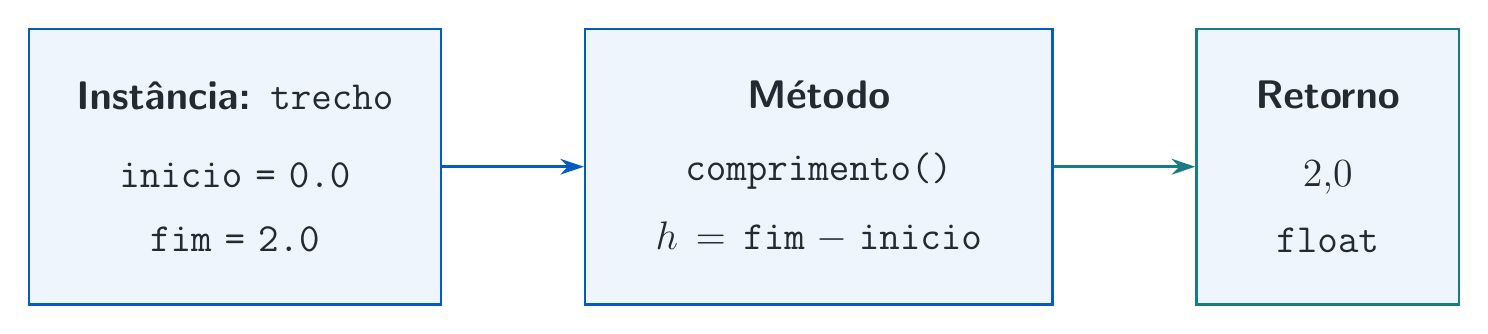
\begin{tikzpicture}
  \node[box,text width=46mm,minimum height=35mm] (dados) at (0,0) {
    \textbf{Instância: \texttt{trecho}}\\[10pt]
    \texttt{inicio = 0.0}\\[5pt]
    \texttt{fim = 2.0}
  };
  \node[box,text width=53mm,minimum height=35mm,right=18mm of dados] (metodo) {
    \textbf{Método}\\[8pt]
    \texttt{comprimento()}\\[7pt]
    $h = \mathtt{fim}-\mathtt{inicio}$
  };
  \node[box,draw=teal,text width=27mm,minimum height=35mm,right=18mm of metodo] (resultado) {
    \textbf{Retorno}\\[10pt]
    $2{,}0$\\[6pt]
    \texttt{float}
  };
  \verificarsetadireita{dados}{metodo}
  \verificarsetadireita{metodo}{resultado}
  \draw[flow] (dados.east) -- (metodo.west);
  \draw[flow,draw=teal] (metodo.east) -- (resultado.west);
\end{tikzpicture}
\end{document}
